\documentclass{if-beamer}

% --------------------------------------------------- %
%                  Presentation info	              %
% --------------------------------------------------- %
\title[Lecture 7]{Lecture 7 }
\subtitle{Namespaces, Variable scopes, control structures, and functions}
\author{Instructor: Ashley Gannon}
\date{ISC3313 Fall 2021}
\logo{

\includegraphics[scale=0.08]{figures/FSULogo.png}
}
\subject{Presentation subject}

% --------------------------------------------------- %
%                    Title + Schedule                 %
% --------------------------------------------------- %
\begin{document}

\begin{frame}
  \titlepage
\end{frame}
% --------------------------------------------------- %
%                      Presentation                   %
% --------------------------------------------------- %
\section{Namespaces}

\begin{frame}
\frametitle{Namespaces}
There are three main namespaces used in C++:
\begin{enumerate}
	\item \texttt{std}: All library entities are defined within namespace \texttt{std}. This includes namespaces nested within namespace \texttt{std}.
	\item \texttt{abi}: Specifies a number of type and function.
	\item \texttt{\_\_gnu\_}: Indicating one of several GNU extensions. Choices include \texttt{\_\_gnu\_cxx}, \texttt{\_\_gnu\_debug}, \texttt{\_\_gnu\_parallel}, and \texttt{\_\_gnu\_pbds}. 
\end{enumerate}
\vspace{5pt}
We'll look more closely at \texttt{std}.
\end{frame}

\begin{frame}
\frametitle{Namespace \texttt{std} for \texttt{iostream}}
\texttt{iostream} is a header that defines the standard input/output stream objects:
\begin{block}{\texttt{cin}}
	Standard input stream
\end{block}
\begin{block}{\texttt{cout}}
	Standard output stream
\end{block}
\begin{block}{\texttt{cerr}}
	Standard error stream
\end{block}
\begin{block}{\texttt{clog}}
	Standard output stream for logging
\end{block}
\vspace{3pt}
As noted in the last slide, all library components of \texttt{iostream} are defined in the namespace \texttt{std}. In order to use the objects in \texttt{iostream}, you must do one of two things:
\begin{enumerate}
	\item Use a \textit{using} declaration in your header file. \\ i.e. \texttt{using namespace std}.
	\item Use a fully qualified library name for each call. \\ i.e \texttt{std::cout} or \texttt{std::cin}
\end{enumerate}
\end{frame}

\begin{frame}
\frametitle{Revisiting "Hello world!" using \texttt{iostream}}
\begin{minipage}[t]{0.5\textwidth}
	\textbf{Option 1:}\\
	{\texttt{}}\\
	{\texttt{}}\\
	{ \texttt{\#include <iostream>}} \\
	{\texttt{}}\\
	{ \texttt{using namespace std;}} \\
	{\texttt{}}\\
	{ \texttt{int main()}} \\
	{ \texttt{\{}} \\
	{ \texttt{\quad \quad  cout<<"Hello world!"<<endl;}} \\
	{ \texttt{\}}} \\
\end{minipage}
\begin{minipage}[t]{0.8\textwidth}
	\textbf{Option 2:}\\
	{\texttt{}}\\
	{\texttt{}}\\
	{ \texttt{\#include <iostream>}} \\
	{\texttt{}}\\
	{\texttt{}}\\
	{\texttt{}}\\
	{ \texttt{int main()}} \\
	{ \texttt{\{}} \\
	{ \texttt{\quad \quad  std::cout<<"Hello world!"<<std::endl;}} \\
	{\footnotesize \texttt{\}}} \\
\end{minipage}

\end{frame}


\section{Variable scope}

\begin{frame}
\frametitle{What is the scope of a variable?}
\vspace{1cm}
We've seen how to declare different types of data, or variables. Are
variables automatically recognized in every part of the program?\\
{\footnotesize \texttt{\#include <iostream>}} \\
{\footnotesize \texttt{}}\\
{\footnotesize \texttt{using namespace std;}} \\
{\footnotesize \texttt{int main()}} \\
{\footnotesize \texttt{\{}} \\
{\footnotesize \texttt{\quad \quad bool a = true;}} \\
{\footnotesize \texttt{\quad \quad if (a)}} \\
{\footnotesize \texttt{\quad \quad \{}} \\
{\footnotesize \texttt{\quad \quad \quad \quad cout << a << endl;}} \\
{\footnotesize \texttt{\quad \quad \}}} \\
{\footnotesize \texttt{\}}} \\
In this case the variable \texttt{a} is obviously known inside the
conditional statement.
\end{frame}

\begin{frame}
\frametitle{What is the scope of a variable}
\vspace{1cm}
In the following case, is the variable \texttt{b} known outside of the
conditional statement? \\
{\footnotesize \texttt{\#include <iostream>}} \\
{\footnotesize \texttt{}}\\
{\footnotesize \texttt{using namespace std;}} \\
{\footnotesize \texttt{int main()}} \\
{\footnotesize \texttt{\{}} \\
{\footnotesize \texttt{\quad \quad bool a = true;}} \\
{\footnotesize \texttt{\quad \quad if (a)}} \\
{\footnotesize \texttt{\quad \quad \{}} \\
{\footnotesize \texttt{\quad \quad \quad \quad double b = 15.0;}} \\
{\footnotesize \texttt{\quad \quad \}}} \\
{\footnotesize \texttt{\quad \quad cout << b << endl;}} \\
{\footnotesize \texttt{\}}} \\
\end{frame}

\begin{frame}
\frametitle{What is the scope of a variable}
\vspace{1cm}
Initialization should be done in the same scope that the variable is
needed: \\
{\footnotesize \texttt{\#include <iostream>}} \\
{\footnotesize \texttt{}}\\
{\footnotesize \texttt{using namespace std;}} \\
{\footnotesize \texttt{int main()}} \\
{\footnotesize \texttt{\{}} \\
{\footnotesize \texttt{\quad \quad bool a = true;}} \\
{\footnotesize \texttt{\quad \quad double b;}} \\
{\footnotesize \texttt{\quad \quad if (a)}} \\
{\footnotesize \texttt{\quad \quad \{}} \\
{\footnotesize \texttt{\quad \quad \quad \quad b = 15.0;}} \\
{\footnotesize \texttt{\quad \quad \}}} \\
{\footnotesize \texttt{\quad \quad cout << b << endl;}} \\
{\footnotesize \texttt{\}}} \\
\end{frame}

\begin{frame}
\frametitle{Local variables versus global variables}
This brings up the concept of variable scope, and local versus global
variables.
\begin{itemize}
\item A local variable lives within the block of code, denoted by
\texttt{\{ \}} symbols, that it is declared in. It will also exist in
any new block that is declared within the original block (like
the first example).
\item A global variable is known to every part of the program.
\end{itemize}
\end{frame}

\begin{frame}
\frametitle{Declaring global variables}
Global variables can be declared outside of the \texttt{main()} function: \\
{\footnotesize \texttt{double b = 15.0;}} \\
{\footnotesize \texttt{int main()}} \\
{\footnotesize \texttt{\{}} \\
{\footnotesize \texttt{\quad \quad cout << b << endl;}} \\
{\footnotesize \texttt{\}}} \\
This gives us 15.0 as output.
\end{frame}

\begin{frame}
\frametitle{Declaring global variables}
\vspace{1.5cm}
They can be modifed as well. What does the following program output? \\
{\footnotesize \texttt{double b = 15.0;}} \\
{\footnotesize \texttt{int main()}} \\
{\footnotesize \texttt{\{}} \\
{\footnotesize \texttt{\quad \quad cout << b << endl;}} \\
{\footnotesize \texttt{\quad \quad b = 10;}} \\
{\footnotesize \texttt{\quad \quad cout << b << endl;}} \\
{\footnotesize \texttt{\}}} \\
\end{frame}

\begin{frame}
\frametitle{Declaring global variables}
\vspace{1.5cm}
They can be modifed as well. What does the following program output? \\
{\footnotesize \texttt{double b = 15.0;}} \\
{\footnotesize \texttt{int main()}} \\
{\footnotesize \texttt{\{}} \\
{\footnotesize \texttt{\quad \quad cout << b << endl;}} \\
{\footnotesize \texttt{\quad \quad b = 10;}} \\
{\footnotesize \texttt{\quad \quad cout << b << endl;}} \\
{\footnotesize \texttt{\}}} \\
This gives us 15.0 as output, followed by 10.0.
\end{frame}

\section{Control structures}

\begin{frame}
\frametitle{If statements}
\vspace{2cm}
We've seen how a basic \texttt{if} statement works, but we can add more
than one condition:
\begin{figure}
\center
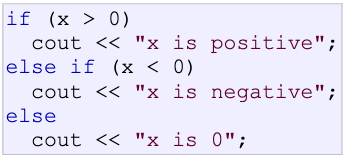
\includegraphics[width=0.6\textwidth]{figures/if.png}
\end{figure}
\end{frame}

\begin{frame}
\frametitle{While loop}
\vspace{2cm}
The while loop executes a block of code until some condition is satisfied:
\begin{figure}
\center
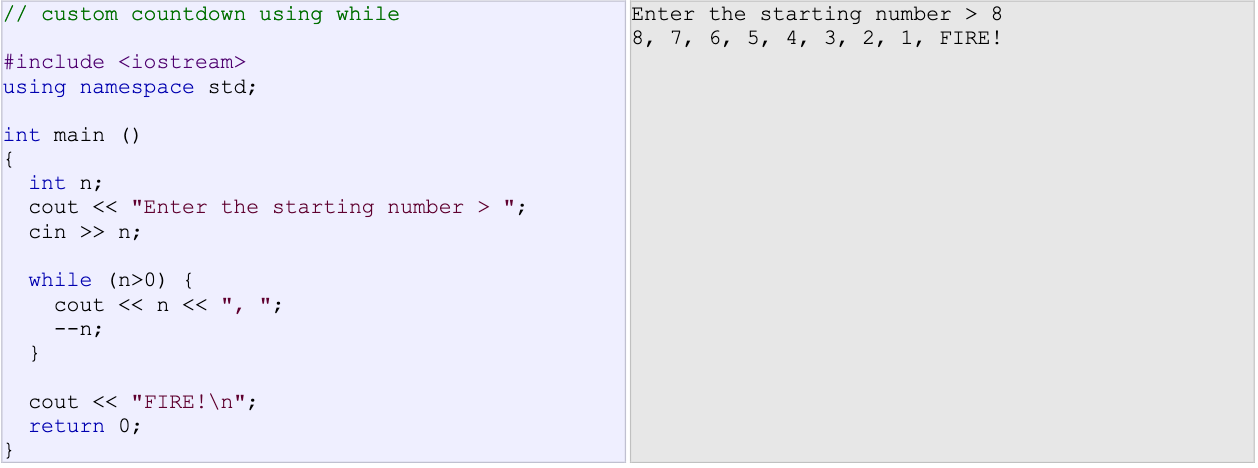
\includegraphics[width=0.95\textwidth]{figures/while.png}
\end{figure}
If the condition is not true initially, the loop will not execute at all.
\end{frame}

\begin{frame}
\frametitle{Do-while loop}
\vspace{2cm}
This type of while loop \textit{always executes at least once}:
\begin{figure}
\center
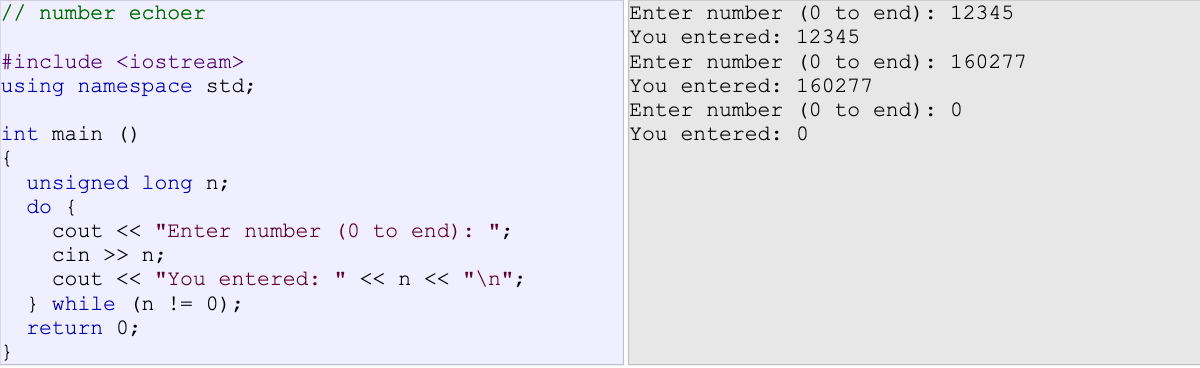
\includegraphics[width=0.95\textwidth]{figures/dowhile.png}
\end{figure}
This is useful if the condition itself is not known until the block of
code executes.
\end{frame}

\begin{frame}
\frametitle{For loop}
\vspace{1cm}
Formally, the pattern of a \texttt{for} loop is: \\
{\footnotesize \texttt{for (initialization; condition; increase) statement;}} \\
The procedure is as follows:
\begin{enumerate}
\item \texttt{initialization} is executed once at the beginning.
This is typically used to set a counter to 0, or the beginning
of an arrary.
\item \texttt{condition} (which is expecting a bool) is checked. If the condition is true, the loop executes at least once.
\item \texttt{statement} is executed. This can be a single line of
code, or many lines of code enclosed in a block \texttt{\{\}}.
\item Whatever code is specified in the \texttt{increase} field is executed. This can be anything.
\end{enumerate}
\end{frame}

\begin{frame}
\frametitle{Jump statements}
There are some special keywords related to loops that are useful:
\begin{itemize}
\item \texttt{break} causes the loop to be exited for any reason
\item \texttt{continue} causes the remainder of a code block to be
ignored, and the \texttt{increase} field to be executed and so
on...
\item \texttt{goto} skips directly to a specified point in the code. There is almost never a good reason to use this.
\item \texttt{exit} terminates the entire code execution, not just a loop.
\end{itemize}
\end{frame}

\begin{frame}
\frametitle{Switch statement}
\vspace{1cm}
A \texttt{switch} statement is used to allow the code execution to
choose between a number of options, similar to \texttt{if-else}
statements.
\begin{figure}
\center
\includegraphics[width=0.3\textwidth]{figures/switch.png}
\end{figure}
\end{frame}

\begin{frame}
\frametitle{Switch statement}
What happens if there are not \texttt{break} statements at the end of each \texttt{case}?
\begin{figure}
\center
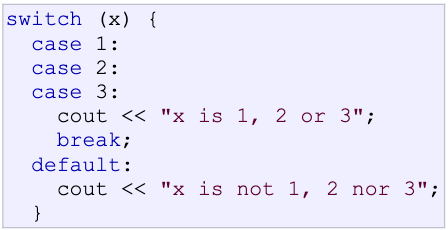
\includegraphics[width=0.6\textwidth]{figures/switch2.png}
\end{figure}
\end{frame}

\section{Functions}

\begin{frame}
\frametitle{Basics of functions}
Functions are like a block of code with additional features:
\begin{itemize}
\item functions return a value, unless \texttt{void} used
\item can return any data type
\item arguments are passed to the function, these can be of any data type
\item arguments can be modifed within the function, or not
\end{itemize}
Their structure looks like: \\
{\footnotesize \texttt{type name (param1, param2, ...) \{ statements \} }}
\end{frame}

\begin{frame}
\frametitle{Calling functions}
Functions must be \textit{declared} before the \texttt{main} program executes.
It can be \textit{defined} anywhere.
\begin{figure}
\center
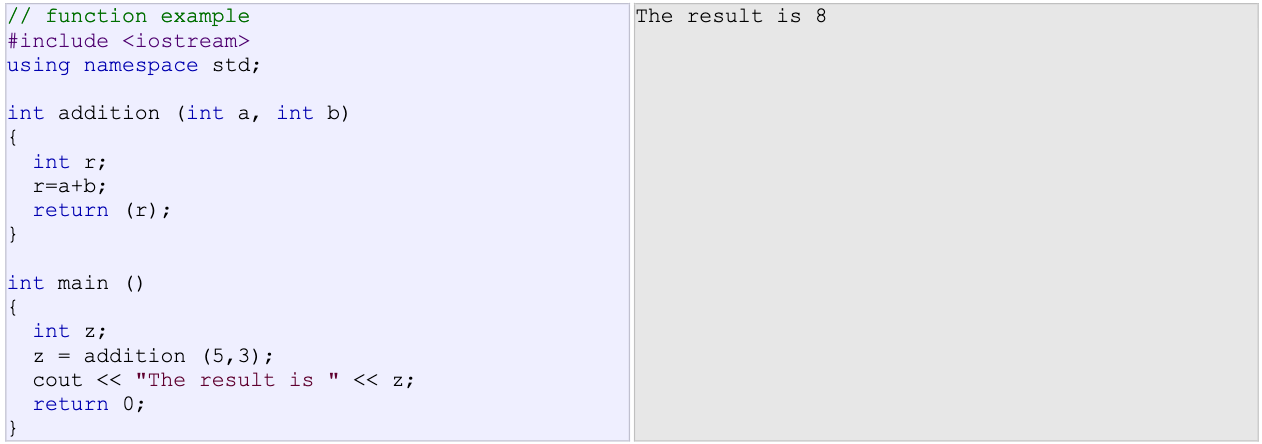
\includegraphics[width=1\textwidth]{figures/func.png}
\end{figure}
Could also just have header at the top: \texttt{int addition(int, int);} and have
the full definition below the \texttt{main} function.
\end{frame}

\begin{frame}
\frametitle{Void functions}
Functions can have a \texttt{void} return type and return nothing.
\begin{figure}
\center
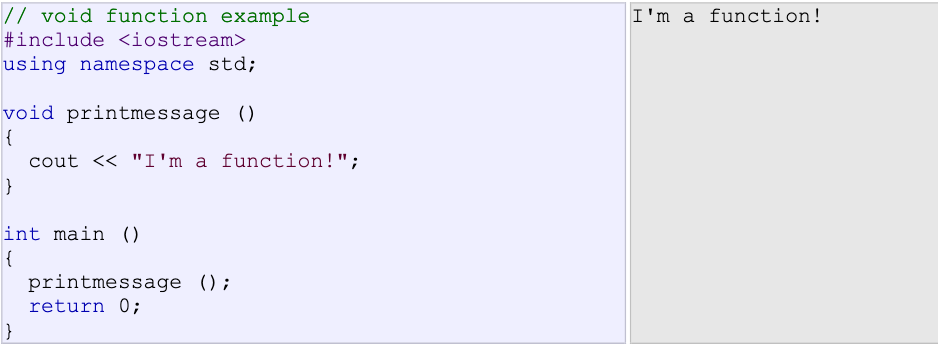
\includegraphics[width=1\textwidth]{figures/void.png}
\end{figure}
\end{frame}

\begin{frame}
\frametitle{Arguments}
Functions can have arguments of any data type. When a function receives
an argument, it makes its own copy of the data. This is known as
\textit{pass-by-value}. Changing the value within the function has no
effect on the value outside of the function.
\end{frame}

\begin{frame}
\frametitle{References}
A reference variable, initialized with an ampersand, becomes an
alternative name for a given variable. It has access to the same address
as the original in memory. \\
{\footnotesize \texttt{double b = 15.0;}} \\
{\footnotesize \texttt{double \&c = b;}} \\
{\footnotesize \texttt{c = 10.0;}} \\
{\footnotesize \texttt{cout << b << endl;}} \\
{\footnotesize \texttt{b = 11.0;}} \\
{\footnotesize \texttt{cout << c << endl;}}
\end{frame}


\end{document}
